\chapter{Power Plant Cost Model Results}\label{ch6:cm_results}

Chapter \ref{ch4:cm_prep} outlined the cost modeling strategy for a hypothetical 5 MW expansion project of the Lightning Dock power plant in Animas Valley, NM. This chapter reviews the results of the different model approaches, explores insights gained from those models, and describes how this approach mitigates risks associated with geothermal production.

\section{Static Model}
\label{ch6:static_mod}

\subsection{Model Selection}

Section \ref{ch4:cm_rev} described the use of brine effectiveness in the cost model for determining the power output of a binary cycle plant for a given production temperature and flow rate. This formulation provides a choice of how to manage the cost model mechanics due to a trade-off between plant capacity and flow rate for a given brine effectiveness (Equation \ref{eq:cm_rev}).

In addition, installation of the Lightning Dock expansion can take place over a variety of different deployment schedules due to the modularity of the system. Rather than drill ten wells and install five binary cycle plants all at once, delaying aspects of the installation can be financially beneficial and less of an initial risk for the project.  

Figure \ref{fig:static_model_compare} shows the results for the pre-set capacity and pre-set flow rate static models for sixty (60) installation schedule permutations. The pre-set capacity model results in project losses of \$20 million or more for all tested installation options. On the other hand, the fixed flow-rate model only drops below \$0 NPV for a handful of project plans, achieving \$3.7 million NPV for the case marked with a red diamond where three (3) modules are installed up front and two (2) additional ones go live after a year of operation. Based on these results, all cost models used in this thesis apply a fixed flow rate per production well and derive electricity generation numbers based on the temperature of the produced brine.

\begin{figure}[!htp]
\centering
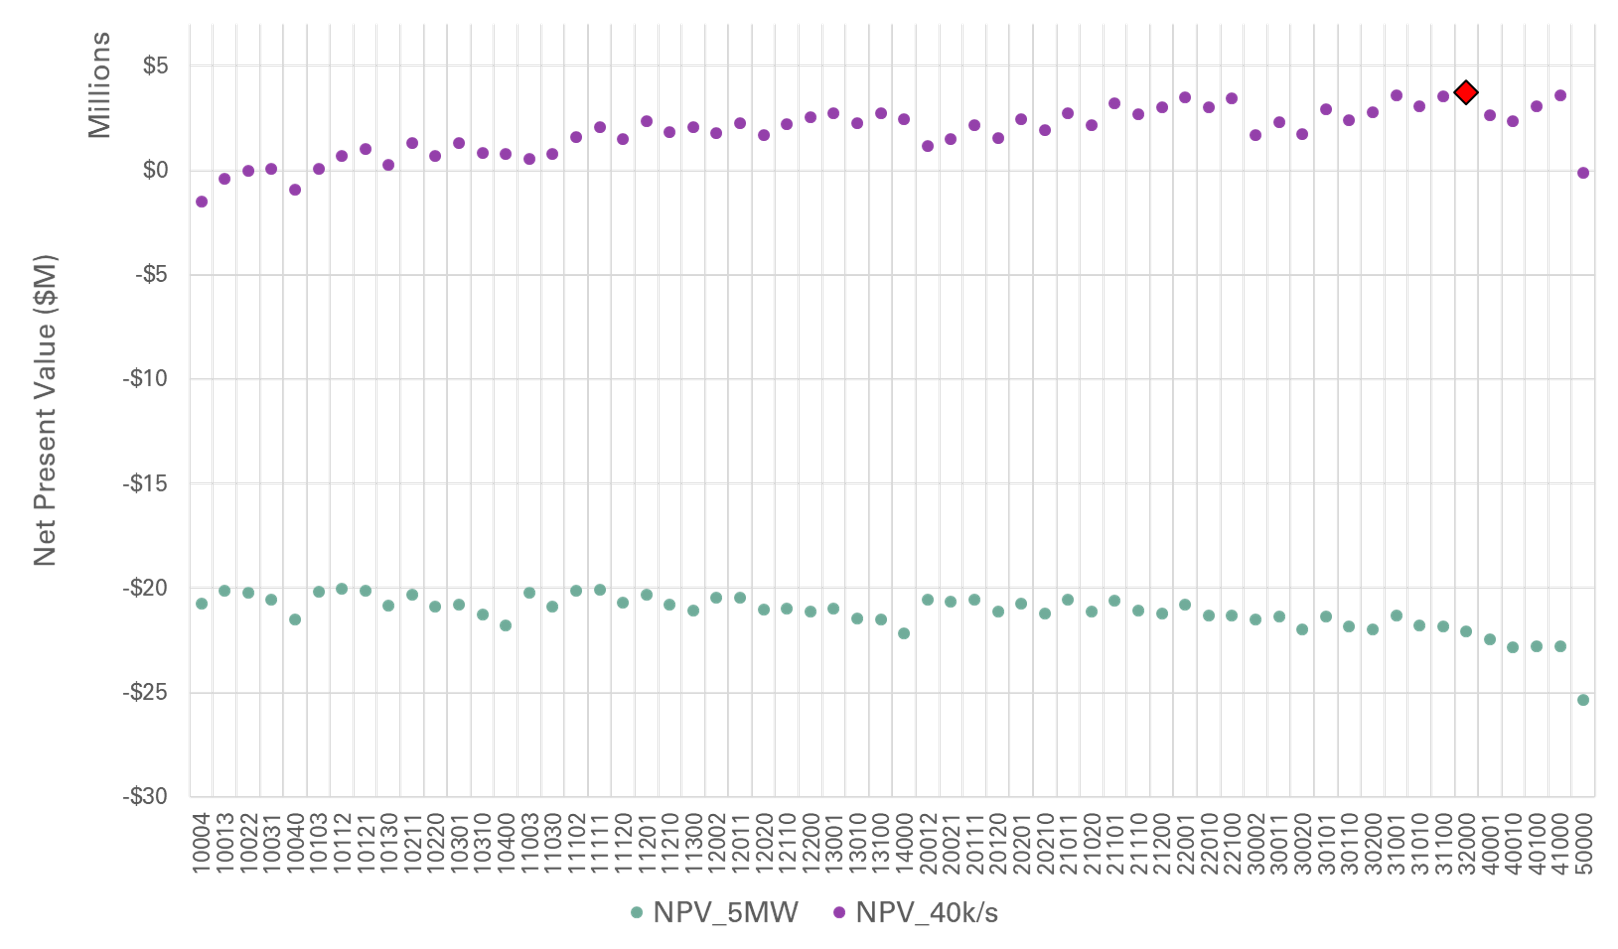
\includegraphics[width=\textwidth]{templates/images/Figure-Static_Model_Construction.png}
\caption[Static cost model comparison]{Static cost model comparison between pre-set aggregate capacity (5 MW target, green) and pre-set flow rate per production well (40 kg/s, purple), plotted against module installation schedule. Both models deploy five modules in all schedule permutations involving up to a five-year period. The red diamond marks the optimal model and power plant expansion plan.}
\label{fig:static_model_compare}
\end{figure}

\subsection{Construction Optimization}

After lifted the fixed-capacity requirement after reviewing results in Figure \ref{fig:static_model_compare}, the hypothetical power plant modules being modeled have an predicted output of 2.1 MW based on the resource and production parameters defined in Section \ref{ch4:cm_npv}. This reduces the required module installation count to a total of three (3) modules based on the original expansion target of $\approx$5 MW. Table \ref{tab:static_optimization} revisits the installation schedule grid search exercise to determine the optimal project plan under these circumstances. At an NPV of \$1.0 million, the best option deploys two (2) modules initially and adds an additional one (1) at the end of the first year. In order to standardize cost models for direct comparison, this installation plan is used for all cost models throughout the rest of this analysis.

\begin{table}[!htp]%{R}{0.4\linewidth}
\centering
\begin{tabular}{|c|c|c|c|}
\hline
\textbf{Year 0} & \textbf{Year 1} & \textbf{Year 2} & \textbf{NPV (\$M)} \\ \hline
3 & 0 & 0 & -\$1.1 \\ \hline
1 & 0 & 2 & -\$0.3 \\ \hline
1 & 1 & 1 & \$0.5 \\ \hline
1 & 2 & 0 & \$0.6 \\ \hline
2 & 0 & 1 & \$0.6 \\ \hline
2 & 1 & 0 & \$1.0 \\ \hline
\end{tabular}
\caption[Static model module installation schedule]{Grid search for the optimal power plant installation schedule based on the static cost model. Values are in \$M, where M is millions.}
\label{tab:static_optimization}
\end{table}

\subsection{Statistics}

\begin{table}[!htp]
\centering
\begin{tabular}{|l|c|}
\hline
\textbf{Static Model Statistics} & \textbf{\$M} \\ \hline
NPV & \$1.0 \\ \hline
\end{tabular}
\caption[Static model statistics]{Static model statistics. NPV is reported in \$M, where M is millions.}
\label{tab:static_mod_stats}
\end{table}

\section{Probabilistic Model}



Common methods for evaluating the ensemble include building an NPV histogram, constructing a cumulative distribution function (target curve), and averaging the results together for Expected Value of NPV (ENPV). Other interesting metrics for model comparison include standard deviation of NPV, extreme cases like P$_{05}$ and P$_{95}$ results, and a direct comparison to the deterministic NPV (NPV$_{det}$). These 



\section{Recap}